\section{Practical Advantages of Open Source}\frame{\sectionpage}

\begin{frame}{Software for Freedom vs. Freedom for Software}
\begin{minipage}{0.5\textwidth}
\begin{itemize}
  \item Needs fulfilled by free software
    \begin{itemize}
      \item a need for software
      \item a need for ethical software and practices
      \end{itemize}
   \item Stallman's emphasis on a ``free digital society''
   \item Consequentialist stance on free software
    \begin{itemize}
      \item open source vs. free software
      \item a less radical approach
      \item weighing the utility of open source
      \item need-driven software (Bisson, 2007, p. 17) 
    \end{itemize}
   \end{itemize}
\end{minipage}
\begin{minipage}{0.45\textwidth}
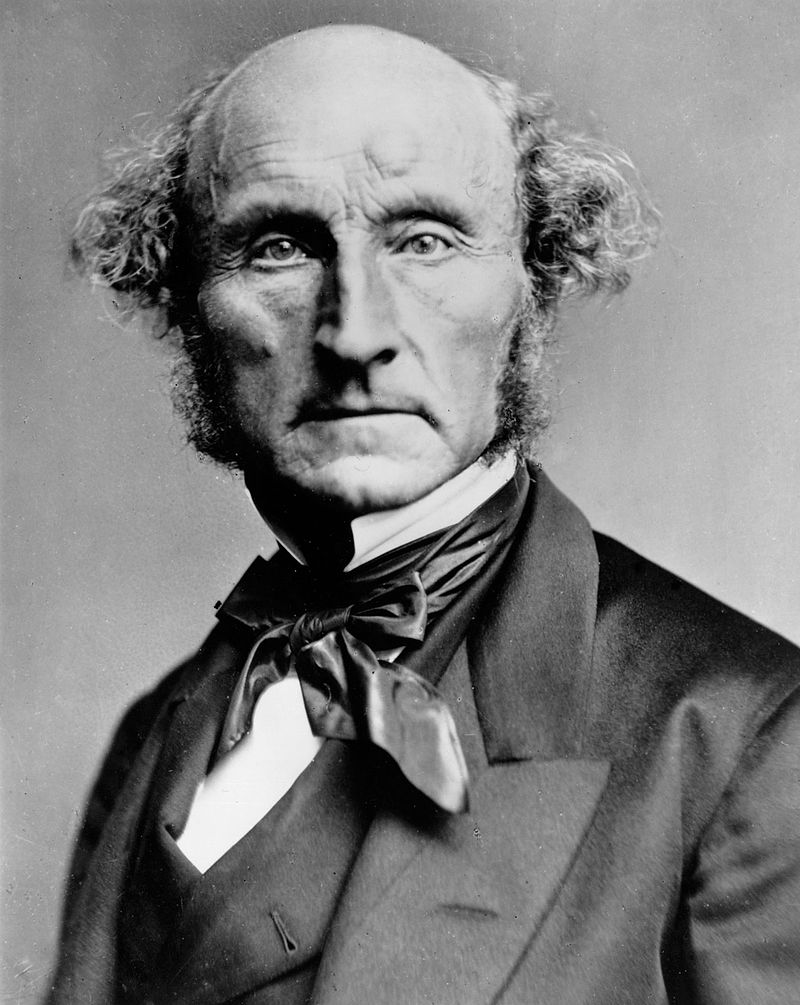
\includegraphics[width = 0.75\textwidth]{mill.jpg}
\end{minipage}
\end{frame}


\begin{frame}{GNU + Linux, GNU/Linux}
\begin{minipage}{0.5\textwidth}
\begin{itemize}
  \item The GNU operating system
    \begin{itemize}
    \item ``written for your freedom'' (Stallman, 2011, para. 48) 
    \end{itemize}    
  \item The need for a kernel
    \begin{itemize}
      \item 1990: GNU Hurd
      \item 1991: Linux
     \end{itemize}
  \item Fusion of Linux and GNU
    \begin {itemize}
      \item GNU + Linux, or just Linux?
      \item Torvalds vs. Stallman
    \end{itemize}
\end{itemize}
\end{minipage}
\begin{minipage}{0.45\textwidth}

\includegraphics[width = 0.75\textwidth]{tux.png}

\includegraphics[width = 0.75\textwidth]{gnu.png}
\end{minipage}
\end{frame}


\begin{frame}{Linux: open source success principles}
\begin{itemize}
 \item Using / creating the best tools for the job
 \item Not started with open source in mind (Torvalds, 3:30)
 \item Open source contributions
 \begin{itemize}
   \item GPL and copyleft
   \item Collaborative efforts and development
   \item Formation of a communities around open-source code
 \end{itemize}
 \item Flexibility
 \begin{itemize}
   \item Availability of source code promotes reuse
   \item power saving on Linux cellphone benefit Linux supercomputers (Zemlin, 2013, 11:34)
  \end{itemize}
\end{itemize}
\end{frame}


\begin{frame}{Another Success Story - Apache HTTP Server}
\begin{minipage}{0.5\textwidth}
\begin{itemize}
  \item Most popular web server since 1995
  \item Open source project
  \item Inherited the NCSA Common Gateway Interface.
  \item Repurposed software components
    \begin{itemize}
    \item enabling efficient software development (Bison, 2007, p. 17)
    \end{itemize}
\end{itemize}
\end{minipage}
\begin{minipage}{0.45\textwidth}

\includegraphics[width = 0.75\textwidth]{apache.png}
\end{minipage}
\end{frame}
 

\begin{frame}{Preventing Obsolescence}
\begin{itemize}
  
  \item Vendor lock-in
    \begin{itemize}
      \item warned against by Stallman (2011, para. 54)
    \end{itemize}
  \item Proprietary software creates vendor dependency 
    \begin{itemize}
      \item maintenance
      \item updates
      \item support
    \end{itemize}
  \item Case Study: Electronic voting machines (Colannino, 2012, p. 916)
    \begin{itemize}
      \item migration to electronic voting machines
      \item software escrow
      \item code was licensed for testing, not deployment. 
    \end{itemize}
\end{itemize}
\end{frame} 
